\chapter{A gentle introduction to Maple and Matlab}
\label{chap:matlab}


\section{Maple}

\section{Matlab}
The ``Mat'' in Matlab does not stand for ``mathematics'', but for ``matrix''..
$\Rightarrow$ all objects in matlab are matrices of some sort! Keep this in mind when using it.
Matlab is a high level \emph{interpreted} programming language: 
\begin{itemize}
\item a matlab program is typically a set of instructions that are evaluated iteratively;
\item most of the work can be done directly from the command line. For convenience, however, it is possible to store these instructions, if they are going to be used repeatedly, in files.
\end{itemize}

\subsection{Computing iterates}

\frame{\frametitle{Defining a function}
We want to plot the iterates of some function $f$. First, we define the function.
\begin{verbatim}
>> f=inline('r.*x.*(1-x)','x','r')
f =
     Inline function:
     f(x,r) = r.*x.*(1-x)
\end{verbatim}
This defines a function (here, with two arguments, $x$ and $r$), that can then be used:
\begin{verbatim}
>> f(0.2,3.2)
ans =
    0.5120
\end{verbatim}
}

\frame{\frametitle{``;'' hides the result on the command line}
Remark that
\begin{verbatim}
>> f(0.2,3.2)
ans =
    0.5120
\end{verbatim}
but
\begin{verbatim}
>> f(0.2,3.2);
\end{verbatim}
produces no output.
}

\paragraph{Creating a vector}
To create a vector, use the command
\[
x=\textrm{first entry}:\textrm{step}:\textrm{last entry},
\]
or, if entries are a subset of the integers,
\[
x=\textrm{first entry}:\textrm{last entry}.
\]
For example, we want to plot the iterates of the logistic map (see details in Section~\ref{sec:DE_logistic}), so
\begin{verbatim}
x=0:0.01:1;
\end{verbatim}
Note the ``;'': otherwise, we get the full 101 elements vector displayed.

\paragraph{What is the size of .. ?}
As mentioned, in matlab everything is a matrix. For matrix operations, size is important, and it is frequent to make mistakes. To check, {\tt whos} and {\tt size}. {\tt whos} gives a lot of information.
\begin{verbatim}
>> whos x
  Name      Size                 Bytes  Class
  
  x         1x101                  808  double array
Grand total is 101 elements using 808 bytes
\end{verbatim}
Various variables can be listed on the line after {\tt whos}:
\begin{verbatim}
>> whos x k
  Name      Size                  Bytes  Class
  
  k         1x1                       8  double array
  x         1x101                   808  double array
Grand total is 102 elements using 816 bytes
\end{verbatim}
If no variable name is provided, {\tt whos} returns the whole workspace, i.e., all variables and their size in memory.

{\tt size}, on the other hand, is ``attributable''. It can be used like this
\begin{verbatim}
>> size(x)
ans =
     1   101
\end{verbatim}
but, since the result is a vector
\begin{verbatim}
>> [r,c]=size(x)
r =
     1
c =
   101
\end{verbatim}
in which case, $r$ and $c$ take the values of the numbers of rows and columns, respectively.


\frame{\frametitle{Vectorized functions versus nonvectorized functions}
Recall that we wrote
\begin{verbatim}
>> f=inline('r.*x.*(1-x)','x','r')
\end{verbatim}
that is, every multiplication sign took the form \verb!.*! instead of \verb!*!. Here, this is needed: we want to use the \emph{vectorized} form of the function, and be able to pass to $f$ a vector instead of a single value. The \verb!.*! form means that the operation is applied to every entry in the vector/matrix. Same exists for \verb!/! and \verb!^!. It is also possible to use the function {\tt vectorize}, which transforms the function into its vectorized equivalent.
\vskip0.5cm
The result of using this vectorized form is that $f$ will be applied to every entry of $x$, and will produce a vector.
\vskip0.5cm
Vectorized operations have been optimized in matlab, and are extremely fast. When possible, they should be used instead of loops.
}

\frame{\frametitle{Vectorized vs nonvectorized}
Define
\begin{verbatim}
>> f=inline('r.*x.*(1-x)','x','r')
>> g=inline('r*x*(1-x)','x','r')
\end{verbatim}
and for simplicity, consider the vector
\begin{verbatim}
>> x=[1,2];
\end{verbatim}
Then
\begin{verbatim}
>> f(x,3.5)
   g(x,3.5)
ans =
     0    -7

??? Error using ==> inlineeval
Error in inline expression ==> r*x*(1-x)
??? Error using ==> mtimes
Inner matrix dimensions must agree.
\end{verbatim}
}

\frame{\frametitle{Plotting}
Basic plotting is very easy. The format is
\begin{verbatim}
plot(x_axis,y_value)
\end{verbatim}
so, for example (with $f$ as defined above),
\begin{verbatim}
plot(x,f(x,3.4))
\end{verbatim}
(here, ``;'' or not does not matter, as the figure appears in a new window and all that ``;'' changes is the output in the command window).
}

\frame{
\begin{center}
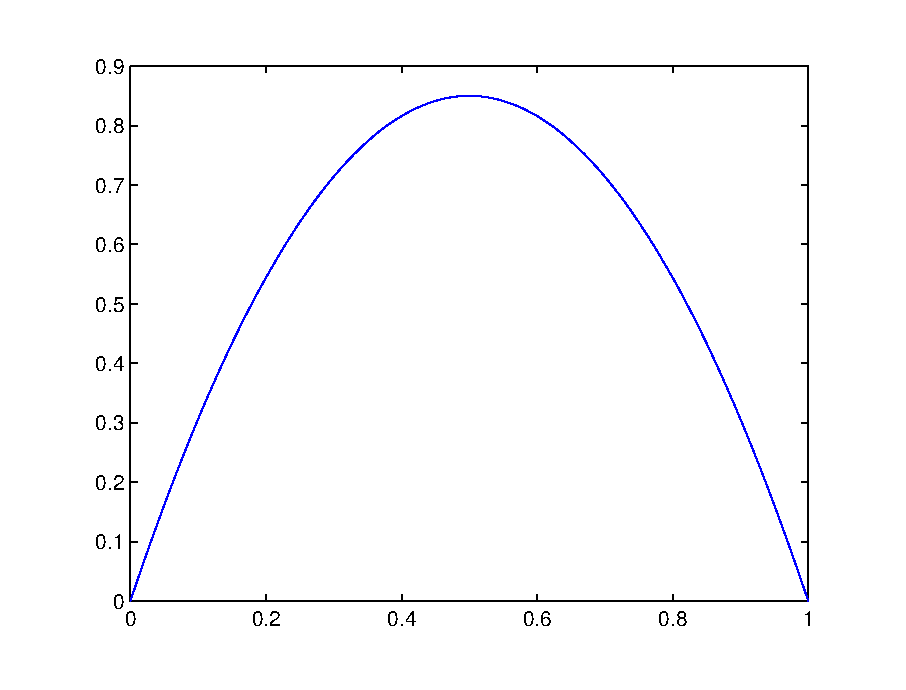
\includegraphics[width=0.5\textwidth]{../figs_01_intro_and_matlab/plot_iterates_1}
\end{center}
}


This is a very basic plot. 
We could want to plot more than one object (for example, the line $y=x$ would be nice).
\begin{verbatim}
plot(x,x,x,f(x,3.4));
\end{verbatim}
Ordering is by pairs: $x_1,f_1(x_1),x_2,f_2(x_2)$. Two elements in a pair {\bf must have} the same number of columns. Different pairs {\bf can have} different numbers of columns. Each element in a given pair can be a point, a vector, a matrix.

We could also want to label the axes.
\begin{verbatim}
xlabel('x');
ylabel('f(x)');
\end{verbatim}
\begin{center}
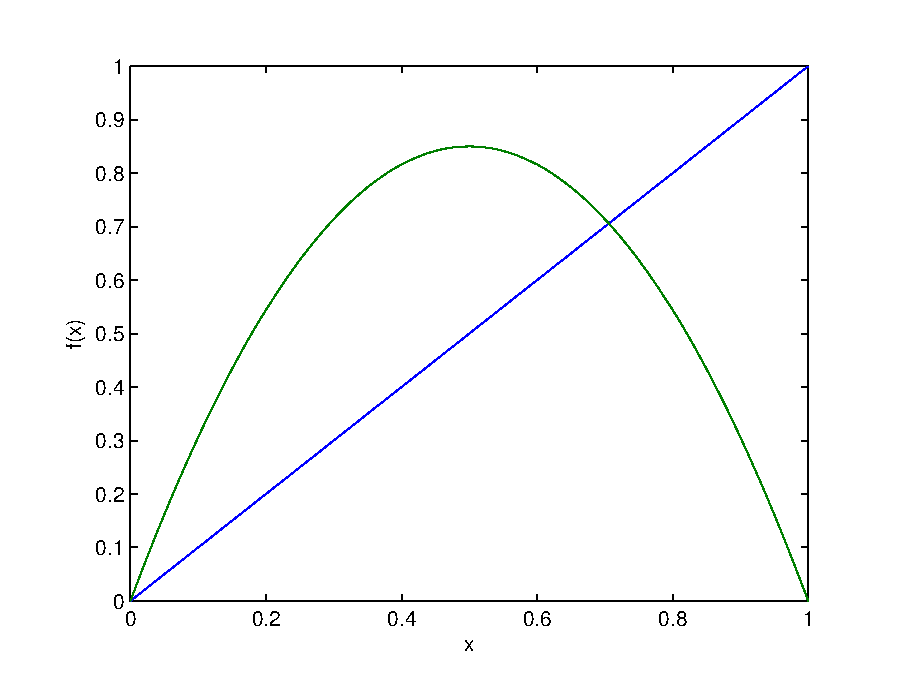
\includegraphics[width=0.5\textwidth]{../figs_01_intro_and_matlab/plot_iterates_2}
\end{center}

\frame{\frametitle{Computing several iterates}
For the moment, we only have $f(x)$. We want $f^n(x)$, for a given $n$. Several ways.
\begin{itemize}
\item Taking for example $r=3.5$, use
\begin{verbatim}
f(f(x,3.5),3.5)
\end{verbatim}
\item The downside to this method is that matlab does not allow to formally define $f^n$, so tricks have to be used for larger values of $n$, for example, produce a string containing the command 
\begin{verbatim}
f(f(f(f(f(x,3.5),3.5),3.5),3.5),3.5)
\end{verbatim}
and evaluate it. This is feasible but complicated.
\item Another method consists in using the result found at the previous step to evaluate the next. We do this now.
\end{itemize}
}


\frame{\frametitle{Automatic resizing of vectors and matrices}
We are going to use a very nice feature of matlab: adding elements to a vector, or rows/columns to a matrix, is automatic. Suppose for example that we had defined $x$ as
\begin{verbatim}
x=0:0.01:0.5;
\end{verbatim}
Then 
\begin{verbatim}
x=[x,0.51:0.01:1];
\end{verbatim}
would produce the vector $x$ as we had earlier.
}

\noindent{\bf Be careful!} Note that the command was
\begin{verbatim}
x=[x,0.51:0.01:1];
\end{verbatim}
that is, the old and new entries were separated by a ``,''. This is \emph{horizontal concatenation}. The command with a ``;'' tries to add a new row. In our case, we get
\begin{verbatim}
>> z=[z;0.51:0.01:1]
??? Error using ==> vertcat
All rows in the bracketed expression must have the same 
number of columns.
\end{verbatim}
because we are trying to add a row of 50 elements to a row of 51 elements. But
\begin{verbatim}
>> z=[z;0.51:0.01:1.01]
\end{verbatim}
works, and gives a $2\times 51$ matrix.


Here, we are going to use the latter form of the command, and add each successive iterate to a solution matrix $M$.
First, define an empty matrix,
\begin{verbatim}
M=[];
\end{verbatim}
Then we need to loop from 1 to $n$, where $n$ is the iterate that we want. 

\frame{\frametitle{Loops}
The command uses the same type of syntax as the creation of a vector: to loop from $4$ to $12$ by steps of 1,
\begin{verbatim}
for i=4:12,
   command(s) to be repeated, maybe using the value i
end;
\end{verbatim}
whereas to loop by non-unit or non-integer steps, say from 4 to 12 by steps of 1.35,
\begin{verbatim}
for i=4:1.35:12,
   command(s) to be repeated, maybe using the value i
end;
\end{verbatim}
Note that in that case, the last $i$ is equal to $10.75$, not $12$, since $10.75+1.35=12.1>12$. The same is true when using non-unit steps to create vectors.
}

\frame{\frametitle{Accessing matrix elements}
Suppose that $M$ is an $m\times n$-matrix. Then
\begin{itemize}
\item {\tt M(i,j)} is the element on the $i$th row and $j$th column.
\item {\tt M(i,:)} is the $i$th row.
\item {\tt M(:,j)} is the $j$th column. 
\item {\tt M(end,:)} is the last row of $M$ ({\tt end} is a reserved word which always points to the last valid index in a given matrix dimension).
\item {\tt M(:,end)} is the last column of $M$.
\item {\tt M(end,1:10)} are the first 10 entries in the last row of $M$.
\item {\tt M(1:2,3:5)} is the submatrix of $M$ consisting of rows 1 and 2 and columns 3 to 5 of $M$.
\end{itemize}
}


\frame{\frametitle{Back to the iterates}
After some thought, we realize that we will need to go back one iterate. So instead of starting with empty matrix $M$, fill the first row of $M$ with first iterate, and start at iterate 2.
\begin{verbatim}
n=10;
r=3.5;
M=f(x,r);
for i=2:n,
    M=[M;f(M(end,:),r)];
end;
plot(x,M);
\end{verbatim}
This plots all the iterates to $n$. The result is a bit crowded, as can be seen in Figure~\ref{fig:10_iterates_logistic}.
\begin{figure}[htbp]
\begin{center}
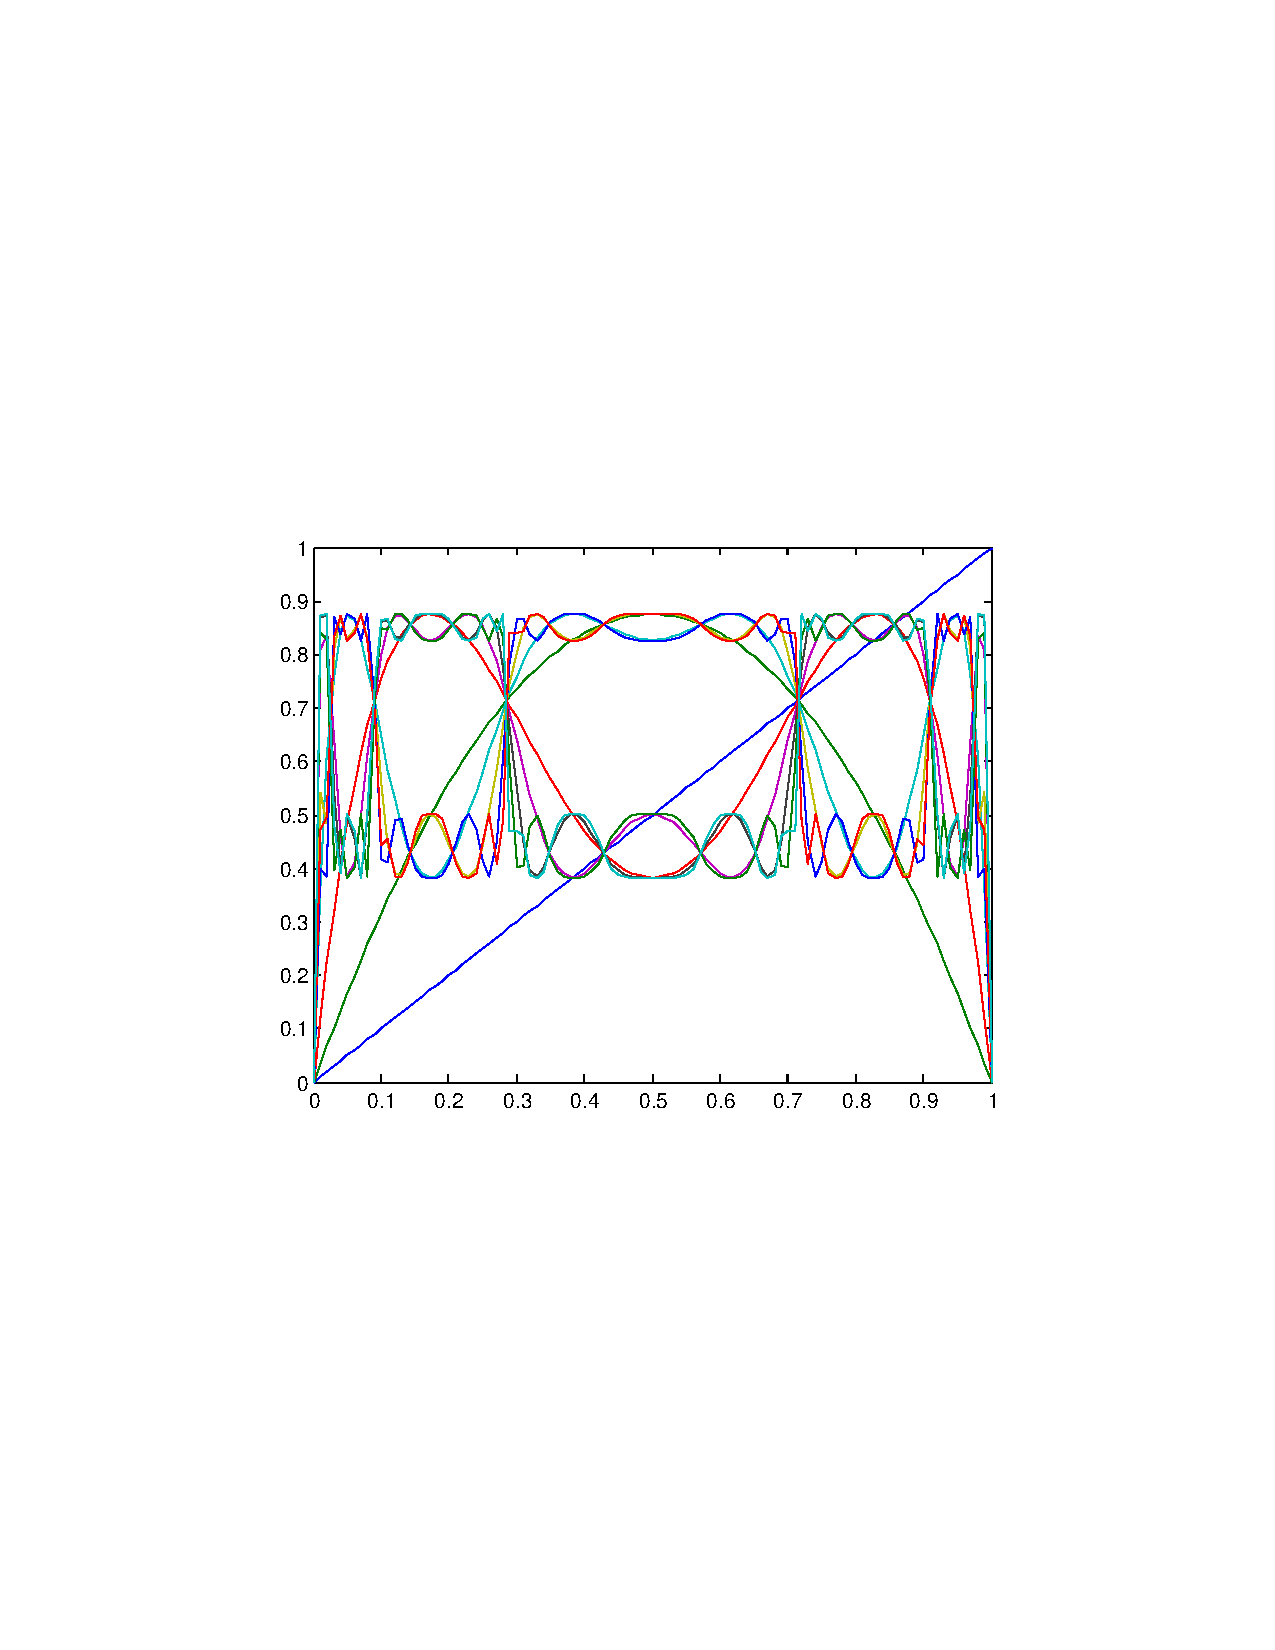
\includegraphics[width=0.5\textwidth]{../figs_01_intro_and_matlab/plot_iterates_3}
\caption{Plot of the first 10 iterates of the logistic map.}
\label{fig:10_iterates_logistic}
\end{center}
\end{figure}


\subsection{Numerical simulation of differential equations}

We want to compute the numerical solution to the logistic equation, which is given by
\begin{equation}\label{eq:ode_logistic_ident}
N'=rN\left(1-\frac NK\right),
\end{equation}
with $r$ the intrinsic growth rate of the population and $K$ the carrying capacity (see Chapter~\ref{chap:single_pop_growth} for details).
There are many ways to do this.
We can use, for example,
\begin{itemize}
\item matlab
\item octave
\item scilab
\item maple
\item mathematica
\item many others..
\end{itemize}
We recommend using matlab, octave or scilab are recommended because of their ``philosophy'',
which is very close to the ``natural'' way one proceeds with an ode. Note also that these programs are geared toward numerical simulations, and are therefore very efficient in that context.

A brief reminder about Euler's method helps to understand the above remark about the ``philosophy'' of the programs. The solution to the initial value problem
\begin{align*}
x' &= f(t,x) \\
x(t_0) &= x_0
\end{align*}
can be approximated numerically by the following sequence:
\begin{align*}
t_{k+1} &= t_k+h \\
x_{k+1} &= x_k+hf(t_k,x_k)
\end{align*}
for a time step $h>0$ and with first term $(t_0,x_0)$.
The techniques (a.k.a. ``numerical solvers'') in matlab are much more advanced, but the idea is the same: approximate the solution to an ODE by using a numerical algorithm that uses information on the ``shape'' of the vector field.
We need two files:
\begin{enumerate}
\item a RHS function defining $f(t,x)$
\item a function or command line statement that ``calls'' the RHS function with a numerical solver
\end{enumerate}
For the logistic equation \eqref{eq:ode_logistic_ident}, we could define the following function:
\begin{verbatim}
function dN=rhs_logistic(t,N,p)
% This function returns the value of dN/dt 
% at the point (t,N), using parameters in the 
% structure p

dN=p.r*N*(1-N/p.K);
\end{verbatim}
which we save in a file called, say, \verb%rhs_logistic.m%. Note that {\tt t} is required in the function arguments even if not used in the RHS function, i.e., even if $f$ is autonomous.

In our code above, the variable {\tt p} is defined as a \emph{structure}. This is a very useful construct in many programming languages. Think of it as a \emph{container}:
\begin{verbatim}
>> p.K=100;
>> p.r=2;
>> p
p =
    K: 100
    r: 2
\end{verbatim}
Pros: {\tt p} is passed to the function as one parameter, instead of a list of parameters. Cons: do not forget {\tt p.} in front of the parameter.
We will see later why structures are useful

Once the right hand side function is set up, we need to invoke the numerical solver.
The call is of the form (from the help): 
\begin{verbatim}
ode23, ode45, ode113, ode15s, ode23s, ode23t, ode23tb

Solve initial value problems for ordinary differential 
equations

Syntax
[T,Y] = solver(odefun,tspan,y0)
[T,Y] = solver(odefun,tspan,y0,options)
[T,Y,TE,YE,IE] = solver(odefun,tspan,y0,options)
sol = solver(odefun,[t0 tf],y0...)

where solver is one of ode45, ode23, ode113, ode15s, 
ode23s, ode23t, or ode23tb
\end{verbatim}
Typically, you can use {\tt ode45}


\frame{\frametitle{Computing the numerical solution to the logistic}
We call our solver as follows:
\begin{verbatim}
tspan=[1790 2000]; %The time span of the solution
IC=3.929;          %The initial condition (in 1790)
p.K=300;           %Set the parameters
p.r=0.5;
[t,N]=ode45(@rhs_logistic,tspan,IC,[],p);
\end{verbatim}
(The one before last argument, {\tt []}, represents the options structure. Here we are not modifying any option, and so pass an empty vector)
\vskip0.5cm
Save this file as, say, \verb%call_solver.m% 
\vskip0.5cm
After running it, we have a vector {\tt t} of times (covering {\tt tspan}) and a vector {\tt N} of solution
}

\frame[containsverbatim]{\frametitle{Plotting the solution}
\begin{verbatim}
plot(t,N)
\end{verbatim}
gives
\begin{figure}[htbp]
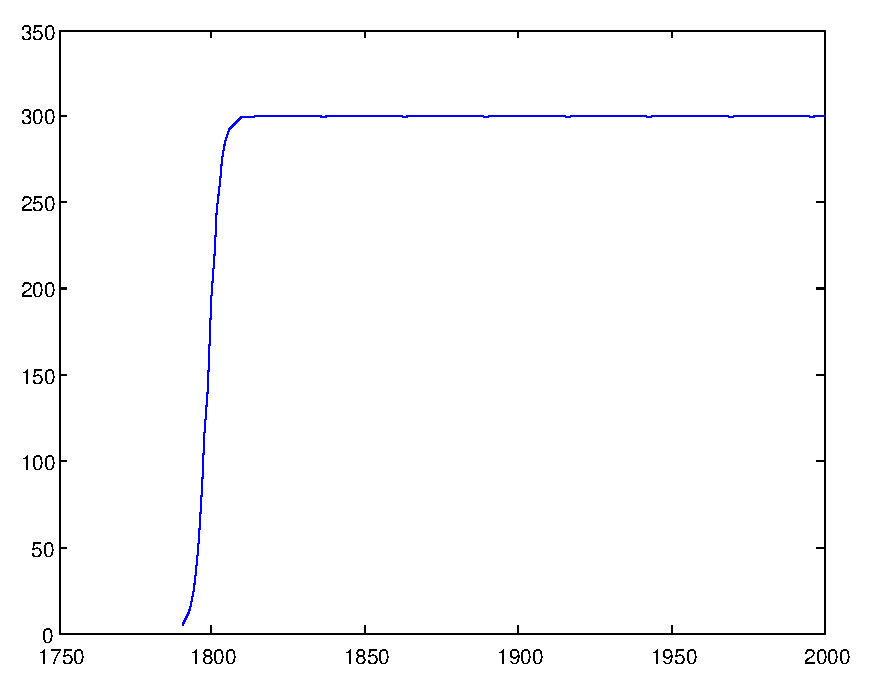
\includegraphics[width=0.7\textwidth]{../figs_09_parameter_identification/fig_logistic_ode_1}
\end{figure}
}

\frame[containsverbatim]{\frametitle{Tightening the $x$-axis}
\begin{verbatim}
plot(t,N)
xlim([t(1) t(end)])
\end{verbatim}
gives
\begin{figure}[htbp]
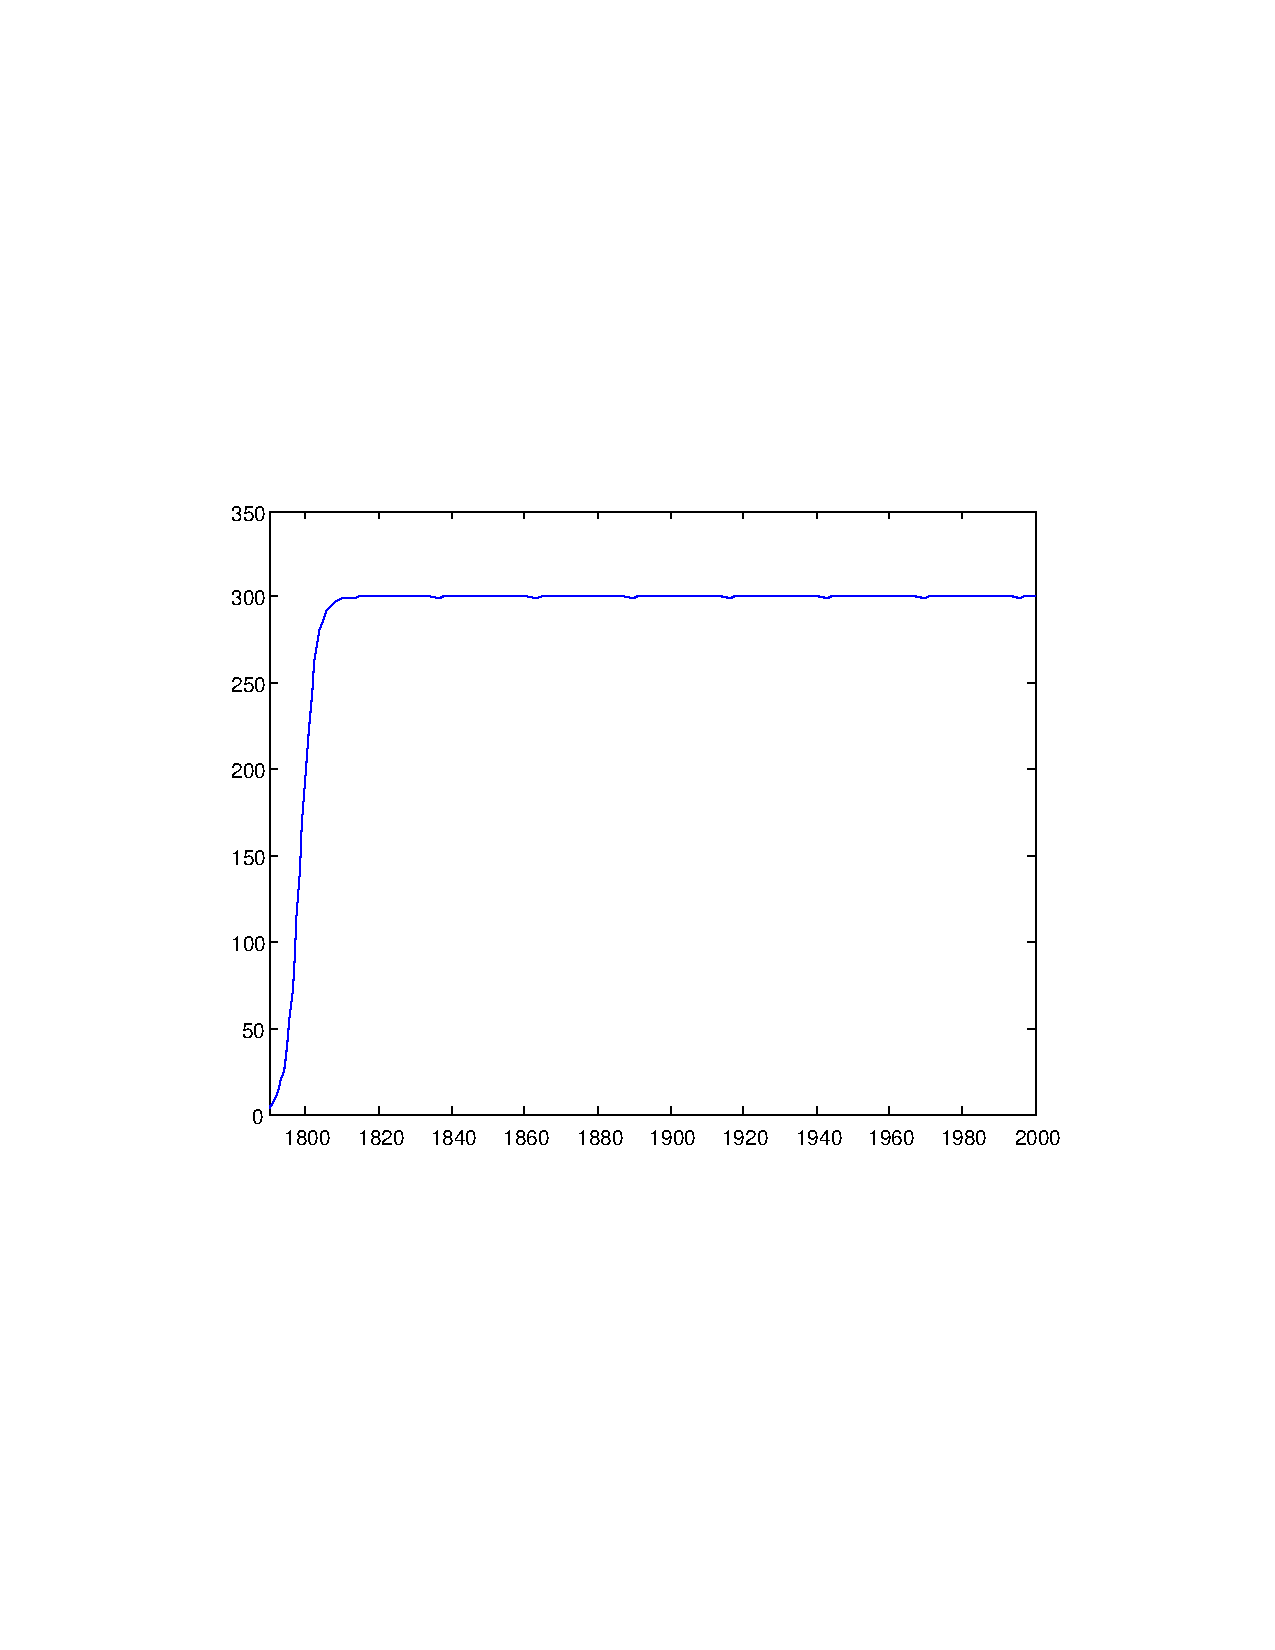
\includegraphics[width=0.7\textwidth]{../figs_09_parameter_identification/fig_logistic_ode_2}
\end{figure}
}

\frame[containsverbatim]{\frametitle{Using Octave}
The syntax in Octave is almost identical to the matlab syntax. In fact, if you use the additional programs in the {\tt forge} repository, a function {\tt ode45} is defined
\vskip0.5cm
However, the functions (in octave) do not implement the use of a parameter by default, so a work-around must be used
\vskip0.5cm
Update: as of V3.0 and using ode45, parameters can be passed and the matlab code given before works, with the following little modification:
\begin{verbatim}
opt=odeset('InitialStep',0.05,'MaxStep',1);
[t,N]=ode45(@rhs_logistic,tspan,IC,opt,p);
\end{verbatim}
which makes sure that the time step does not become too large)
}


\frame[containsverbatim]{\frametitle{Using scilab}
The syntax in scilab differs a little from matlab, so beware.
\begin{verbatim}
function ydot=f(t,y);
ydot=y^2-y*sin(t)+cos(t);
endfunction
\end{verbatim}
}

